
\documentclass[12pt,a4paper]{report}
\usepackage{graphicx}
\usepackage[francais]{babel}
\usepackage[utf8]{inputenc}
\usepackage[T1]{fontenc}
\usepackage{alltt}
\usepackage{fancyhdr}
\setlength{\headheight}{15.2pt}
\pagestyle{fancy}
  
\title{Rapport de soutenance \no{2}} 
\date{}
\author{TeGaSz}
\newcommand{\HRule}{\rule{\linewidth}{0.5mm}}



\begin{document}

\begin{titlepage}



\begin{center}



\textsc{\LARGE PROJET}\\[1.5cm]

\textsc{\Large TeGaSz}\\[0.5cm]


% Title
\HRule \\[0.4cm]
{ \huge \bfseries Rapport de Soutenance 2}\\[0.4cm]
  
\HRule \\[1.5cm]

\includegraphics[width=0.6\textwidth]{./name.jpg}\\[1cm]  
% Author and supervisor
\begin{minipage}{0.4\textwidth}
\begin{flushleft} \large
Julien \textsc{Garagnon}\\
Julien \textsc{Szkudlarek}
\end{flushleft}
\end{minipage}
\begin{minipage}{0.4\textwidth}
\begin{flushright} \large
Maxime \textsc{Templé}\\

\end{flushright}
\end{minipage}

\vfill

% Bottom of the page
{\large 17 avril 2012}

\end{center}

\end{titlepage}
\tableofcontents

\chapter{Introduction}
Ceci est le rapport de soutenance du projet réalisé par l'équipe \emph{TeGaSz}. 
Ce dernier se prénomme \emph{P.R.O.J.E.T} (Programme Radiophonique Orienté Jouant Énormémentsur les Tonalités) et est en définitive un lecteur Audio programmé pour fonctionner sous Fedora. \\
Dans ce rapport, nous allons vous présenter notre projet terminé ainsi
que toute la démarche de sa conception, qu'elle soit intellectuelle, sous forme de recherche ou tout simplement en code pur.

\chapter{Le projet}
\section{Les origines du projet}

Le groupe TeGaSz est un groupe de projet formé en 2012 par trois étudiants
d'EPITA passionnés, dans le but de réaliser pour la fin de l'année un
travail de programmation inédit. Ce programme est un lecteur audio codé
dans la majeure partie en C et en Ocaml. Le projet sera accompagné d'un
site web qui décrira tout au long de l'année l'avancement du projet. Il sera
mis à jour régulièrement après chaque évolution notable. Ce projet sera particuli
èrement diffcile à réaliser au niveau de la programmation : En effet, ce
projet demande des notions particulièrement avancées dans le domaine du
cryptage des fichiers audio. Par exemple, il faudra être capable de distinguer
les en-tête de fichier de type .mp3, ou tout simplement être capable de lire
un son, montrer sons avancement dans le temps, et pourquoi pas, afficher
plusieurs informations sur la musique en cours. C'est pourquoi nous allons
commencer ce projet en progressant étape par étape.

\section{Etude du marché}
Nous nous intéressons principalement aux lecteurs audio libres, puisque c'est à cela que nous espérons arriver. voici quelques uns des logiciels disponibles sur le marché:

\subsubsection{The KMPlayer}

Simple et épuré KMPlayer n'en est pas moins puissant. Ce lecteur Coréen a le vent en poupe et il se dit dans les forums qu'il commence à faire de l'ombre à VLC. Lecteur multimédia, KMPlayer est capable de lire pratiquement tous les formats audio et vidéo nativement. Il est doté d'une très belle interface vraiment simple à  utiliser. A découvrir... Il est gratuit et un patch français est disponible.

\subsubsection{Amarok}

Amarok est un lecteur audio. Il était au départ conçu uniquement pour Linux, mais la migration vers les plateformes Windows et Mac OS X est en cours. C'est\`a ce jour l'un des meilleurs lecteurs audio. 
 Amarok peut lire quasiment n'importe quel type de fichiers audio (MP3, OGG, WMA, FLAC...), permet la création de playlists ce qui le transforme en Jukebox, gère l'édition des tags, grave les CD audio (à condition d'avoir K3B), récupère les pochettes de disques ou les paroles d'un morceau, permet d'uploader votre musique vers de nombreux baladeurs (iPod, Creative NOMAD ou ZEN, Rio Karma...), affiche les informations de Wikipedia sur le groupe que vous écoutez... Bref, Amarok est un outil très puissant.
Il faut disposer d'un moteur de décodage tel que GStreamer ou Xine pour faire fonctionner Amarok : Amarok est en quelque sorte une interface utilisateur. 

\subsubsection{Splayer}

Lecteur multimédia extrêmement léger, Splayer est compact, gratuit, facile à utiliser et capable de lire pratiquement tous les formats audio et vidéo sans avoir besoin de plugins supplémentaires. Il est doté d'une superbe interface que l'on apprécie d'autant plus quand on utilise Splayer pour lire des vidéos. 

\subsubsection{Windows Media Player}

Le format WMA est la réponse de Microsoft au MP3. Face au succès du MP3 et l'engouement des internautes pour ce format, Microsoft a réagi en mettant au point le Windows Media Audio codec en 1999. Les techniques de compression sont semblables à celles utilisées par le standard MP3. Windows Media Player est fourni directement avec Windows depuis Windows 98. Pour obtenir la dernière version, voyez les liens ci-dessous. Windows Media Player permet la lecture des CD audio, des fichiers MP3 et WMA et la visualisation de fichiers vidéo. Il est doté d'un égaliseur 10 bandes, d'un gestionnaire de Playlists qui le transforme en Jukebox. Il permet la compression des fichiers Wave en WMA. On peut aussi procéder à l'extraction des pistes audio d'un CD. Les fichiers obtenus sont directement encodés en WMA (on ne récupère pas les wave). Il existe des skins et des plug-ins pour le transfert vers des baladeurs.

\subsubsection{Winamp}

Premier lecteur MP3 logiciel apparu sur le Web en 1997 et toujours très populaire. Aujourd'hui, Winamp est bien plus qu'un simple lecteur MP3. Il permet la lecture des CD audio, des fichiers MP3, OGG, AAC et WMA sans ajout de plug-ins et ceci pour ne parler que des formats les plus courants. Il peut désormais ripper les pistes d'un CD audio pour les copier sur votre disque dur et graver des CD. Ces deux dernières fonctionnalités sont limitées dans la version gratuite : on peut ripper en x6 et graver en x2 seulement mais c'est possible. Cette limitation ne nous semble pas un gros handicap dans la mesure o\`u il vaut mieux ripper \`a  vitesse lente pour obtenir une bonne qualité d'extraction. Mais revenons \`a  Winamp... Il est doté d'un égaliseur 10 bandes, d'un gestionnaire de Playlists qui le transforme en Jukebox et d'un mini navigateur Web. 
L'ajout de plug-ins étend encore les possibilités de Winamp puisqu'on peut encoder en MP3 ou autre format, visualiser des vidéos au format DivX, lire des fichiers audio de type VQF, Monkey... A tester !

\section{Présentation de l'équipe}
TeGaSz est un projet réalisé par trois étudiants en deuxième année à EPITA.
	\subsection{Maxime Templé}
Il y a maintenant quatre ou cinq ans, j'ai découvert les possibilités que pouvaient donner l'informatique. Malgré quelques notions de C et depuis six mois de Ocaml,et un projet en C\# je n'ai jamais eu l'occasion de m'investir pleinement dans le domaine du son lié à la programmation, mais je compte me servir de ce projet afin d'approfondir mes connaissances dans le domaine.

	\subsection{Julien Garagnon}
Troisième année a l'Epita, troisième spé, et enfin je commence le C. Après l'échec du projet cartographie, j'espère bien me rattraper avec cette fois ci un groupe soudé et motivé. n'ayant pratiquement aucune expérience concernant le son, que ça soit sa lecteur, sa production ou encore sa manipulation, ce projet promet de m'apporter de nombreuses connaissances sur le sujet, connaissances dont je suis toujours avide.

	\subsection{Julien Szkudlarek}
Après un premier projet consistant à réaliser une cartographie 3D avec un grand intérêt principalement lié à la visualisation, celui-ci sera donc un lecteur audio. Il s'annonce tout aussi passionnant car le principe même du projet est un outil très commun et de notre quotidien aujourd'hui. Il va également me permettre de pouvoir approfondir le C que je connais relativement peu. Pouvoir créer son propre lecteur audio est un objectif très stimulant d'autant plus que le sujet est plus libre que le précédent ce qui va permettre une meilleure créativité.

\section{Librairies utilisées}
	\subsection{Fmod}

\begin{center}

\includegraphics[scale =0.5]{fmodex.png}
\end{center}
FMOD est une bibliothèque multiplateforme de gestion du son, pouvant être utilisée au travers de noombreux langages de programmation. Avec le lancement de la version 4.03 la bibliothèque a été renommée FMOD Ex.

	\subsection{GTK}

\begin{center}

\includegraphics[scale =0.5]{GTK.jpg}
\end{center}

GTK+ (The GIMP Toolkit) est un ensemble de bibliothèques logicielles, c'est-à-dire un ensemble de fonctions informatiques, permettant de réaliser des interfaces graphiques. Cette bibliothèque a été développée originellement pour les besoins du logiciel de traitement d'images GIMP. GTK+ est maintenant utilisé dans de nombreux projets, dont les environnements de bureau GNOME, Xfce et ROX.
GTK+ est un projet libre (licence GNU LGPL 2.1) et multiplate-forme.

Même si, au départ GTK+ est écrit en langage C et utilise pourtant le paradigme de la programmation orientée objet. Il est également possible d'utiliser GTK+ dans de nombreux autres langages de programmation: C++ (avec gtkmm), Ada (avec GtkAda), Fortran (avec gtk-fortran), Pascal, PHP, Perl, Ruby, Objective Ocaml, Java, Python, Vala, Seed (JavaScript) ou encore C\# avec la plateforme mono au travers du binding Gtk\#, etc.

\chapter{Le planning}
Pour pouvoir réaliser ce projet dans les temps, nous avons choisi de travailler en groupe au moins une fois par semaine, sur des plages d'horaires communes comme le Vendredi soir ou le jeudi matin. Le reste du travail sera réalisé individuellement par chaque membre de l'équipe en suivant un planning et une répartition organisée des tâches décrite plus bas. Le but de ces réunions hebdomadaires est tout simplement de mettre en commun nos idées et de faire le point sur l'avancée du travail de chacun. Ainsi, chaque semaine un planning pour la semaine suivante sera établi pour chaque membre de l'équipe.

\section{Organisation du travail}

Pour pouvoir réaliser ce projet dans les temps, nous avons choisi de travailler en groupe au moins une fois par semaine, sur des plages d'horaires communes comme le Vendredi soir ou le jeudi matin. Le reste du travail sera réalisé individuellement par chaque membre de l'équipe en suivant un planning et une répartition organisée des tâches décrite plus bas. Le but de ces réunions hebdomadaires est tout simplement de mettre en commun nos idées et de faire le point sur l'avancée du travail de chacun. Ainsi, chaque semaine un planning pour la semaine suivante sera établi pour chaque membre de l'équipe.

\section{répartition des tâches}

Tout au long du semestre, nous nous sommes donnés des tâches précises à faire avancer chacun de notre coté. cependant, le temps avancant et la dead line approchant, chaque personne a quitté son travail pour aller aider un autre membre de l'équipe. Nous pouvons donc dire que tout le monde aura travaillé sur tout le projet.
Dans le projet initial, Julien G devait s'occuper de mettre en place la librairie Fmod, Julien S de l'interfaçage entre le C et le Ocaml et enfin Maxime devait mettre en place 

 graphique.

\section{Le chef de projet}

La personne qui s'occupera tout au long de l'année de la mise en place du projet et de l'organisation des travaux sera Maxime, choisi à l'unanimité. Il sera notre chef de projet, c'est-à-dire le principal intermédiaire entre le jury et le groupe de projet lors des soutenances.

\section{utilisation de git}

\begin{center}

\includegraphics[scale =0.5]{git.png}
\end{center}

il nous fallait un outil fiable afin de partager notre avancé commune. Le gestionnaire de version décentralisé GIT semblait tout destine pour cette tache. Pour cela, nous avons donc créé un dépôt sur le site GitHub qui permet gratuitement d'héberger l'ensemble de nos sources.\\
Git est un logiciel de gestion de versions décentralisé. C'est un logiciel libre créé par Linus Torvalds, le créateur du noyau Linux, et distribué selon les termes de la licence publique générale GNU version 2.


\chapter{Le developpement du projet}
Notre projet s'est développé progressivement. Chaque soutenance était une étape avec de nouvelles améliorations, implémentations et d'autres choses plus ou moins visibles. 
Ces avancées seront développées avec précision dans les chapitres prévus à cet effet.

\section{la première soutenance}

\begin{center}
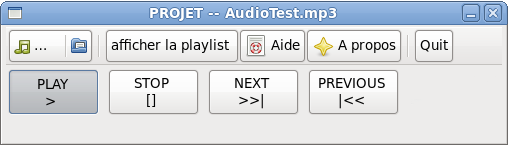
\includegraphics[scale = 0.8]{interface1.png}
\it{ première version du projet}

\end{center}
Lors de cette première soutenance nous nous sommes particulièrement concentré sur l'interfaçage entre le C et le Ocaml parce que cette partie était la plus importante:
Sans elle nous ne pouvions effectuer aucun test! 
Un premier tatonnement sur Fmod aura aussi été fait et l'interface aura été implémentée. 
Au final, nous avions un lecteur audio ne pouvant jouer qu'une seule musique prédéfinie.

\section{la deuxième soutenance}

\begin{center}
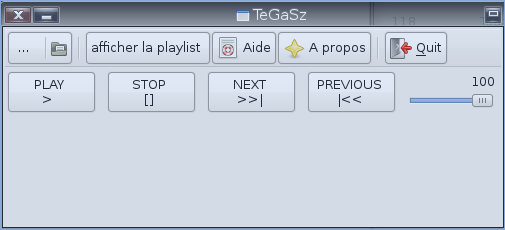
\includegraphics[scale = 0.8]{interface2.png}
\it{ seconde version du projet}
\end{center}


L'interfaçage entre C et Ocaml ayant été implementé pour la première soutenance,  nous pouvions nous concentrer sur le projet en lui-même, à savoir la mise en place de Fmod et son imprecation dans l'interface.
Nous avions donc un lecteur audio plus complexe permettant de charger une chanson, de la lire et de varier le volume.

\section{la soutenance finale}

\begin{center}
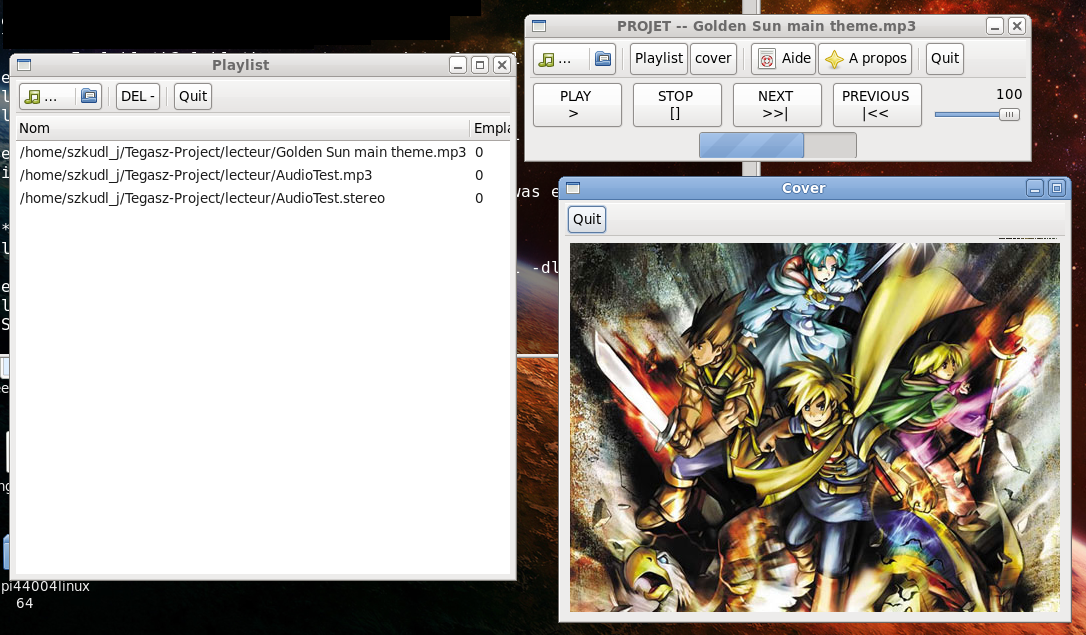
\includegraphics[scale = 0.4]{interface3.png}
\it{visuel final}
\end{center}

\chapter{l'interface}

Pour cette dernière version, le principe de base aura été de repartir à
partir des bases posées dans la deuxième soutenance. Nous avons utilisé nos connaissances acquises dans nos recherches pour réaliser une interface qui correspondait beaucoup plus aux attentes du cahier des charges, Bien que les methodes employées pour la plupart des parties restent fondamentalement les memes, nous avons surtout ajouté des actions plus spécifiques, permettant ainsi une meilleure interconnexion entre les différentes parties du projet.

Pour la fin nous avons mis en place les deux nouvelles fenêtres pour la pochette et la playlist.

\section{description des boutons}

L'interface inclue toutes les fonctions que l'on peut attendre d'un lecteur
audio fonctionnel : 
Nous pouvons sélectionner le fichier à charger,lire ce dernier à l'aide du bouton play, un bouton stop pour arrêter la lecture, une barre de volume pour régler l'intensité du son.

 Il y a aussi deux boutons pour changer de piste, bien qui sont fonctionnels pour cette nouvelle soutenance.

Une des particularité du bouton de lecture est qu'il permet aussi de mettre
en pause la lecture.

 Une fois pressé, il reste enfoncé et ainsi l'utilisateur sait que la piste est lue. S'il est de nouveau cliqué, il ressort et la lecture est mise en pause et peut être reprise au même point.

La sélection du volume se fait par une barre coulissante, avec une indication
numérique du volume actuel pour une plus grande précision. A la base,
le volume est indiqué avec une décimale, ainsi pour raison esthétique, nous
avons préféré ne garder que les entiers.

Pour cette nouvelle soutenance, deux nouveaux boutons sont apparus.  le bouton pour afficher la playlist, qui affiche une nouvelle fenêtre contenant bien entendu la liste de lecture, mais aussi un bouton permettant d'ajouter un morceau à la liste, et un autre pour le supprimer.
le second bouton de l'interface permet d'afficher la pochette de l'album.

En ce qui concerne les autres nouveautés, une barre de défilement a été ajoutée.

\section{Architecture de l'interface}



\begin{center}
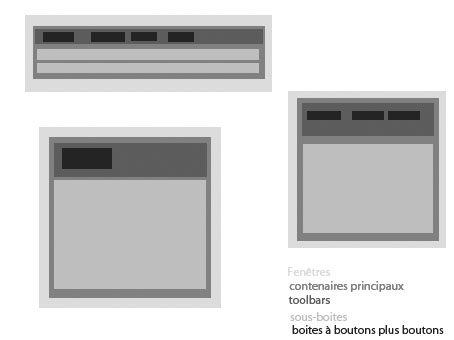
\includegraphics[scale =0.8]{archi.jpg}
\end{center}


Nous pouvons considérer l'interface GTK comme une sorte de Poupée Russe. Il s'agit d'une série de fenêtres et d'imbrications en tout genres.
Tout d'abord nous avons la fenêtre de base, la fenêtre de la playlist et enfin la fenêtre pour la couverture. Contrairement aux deux autres, la première est visible.
Cette dernière contient une boite de boites,contenant elle même une une toolbar, une boite de boutons et une boite de Widgets.La toolbar contient une série d'items contenant chacun un bouton, ou une séparation.
la bouton barre contient les quatres boutons de contrôle et encore une boite de widgets servant à afficher la barre de réglage de volume.

Le troisième élément de  la première boite contient la barre de progression.
une fois cliqué sur le bouton pour afficher la couverture, s'affiche une seconde fenêtre contenant elle aussi un conteneur principal, contenant lui même une toolbar et une boite de fichiers. la toolbar contient une boite de boutons pour afficher le bouton quitter. l'autre boite contient l'image que l'on désire afficher.

Nous procedons de la même façon pour la playlist.


\chapter{Moteur son}

\chapter{l'interface c/Ocaml}
\chapter{ La playlist}
\chapter{la pochette}
\chapter{site web}


\chapter{Conclusion}

\begin{center}

\includegraphics[scale =0.5]{conclu.jpg}
\end{center}
\end{document}
